\documentclass[12pt, a4paper]{article}
\usepackage[utf8]{inputenc}
\usepackage[T1]{fontenc}
\usepackage{amsmath}
\usepackage{graphicx}
\usepackage{hyperref}
\usepackage{fancyhdr}
\usepackage{enumitem}
\usepackage{caption}
\usepackage{subcaption}
\usepackage{xcolor}
\usepackage{geometry}
\usepackage{listings}
\usepackage{float}
\geometry{a4paper, margin=1in}

% Header and Footer
\pagestyle{fancy}
\fancyhf{}
\fancyhead[L]{\textit{MemoVault}}
\fancyhead[R]{\thepage}
\fancyfoot[C]{}
\renewcommand{\headrulewidth}{0.4pt}
\renewcommand{\footrulewidth}{0pt}

% Code listing settings
\lstset{
    basicstyle=\ttfamily\small,
    \begin{itemize}
    \end{itemize}
    frame=single,
    numbers=left,
    numberstyle=\tiny,
}

% Title Page
\title{\textbf{MemVault: A Decentralized Memory Layer for AI-Native Applications}\\
\vspace{0.5cm}
\large Building User-Controlled AI with Privacy-First Architecture}

\author{
Aaron Phan\\
\textit{CommandOSS Labs}\\
\href{mailto:aaron.phan@commandoss.com}{aaron.phan@commandoss.com}
}

\date{December 2025}

\begin{document}

\maketitle
\thispagestyle{empty}

\newpage
\tableofcontents
\thispagestyle{empty}

\newpage
\section{Executive Summary}

MemoVault represents a paradigm shift in human-AI interaction, solving the fundamental conflict between AI personalization and user privacy. As artificial intelligence becomes increasingly central to digital life, current centralized architectures force users into an impossible choice: surrender personal data for intelligent assistance or maintain privacy without personalization.

MemoVault eliminates this false dichotomy through a \textbf{production-ready decentralized memory layer} that enables:

\begin{itemize}
    \item \textbf{True Data Ownership}: Users maintain cryptographic control of their AI interactions and memories through Sui blockchain
    \item \textbf{Privacy-First Personalization}: Sophisticated AI assistance without exposing personal data to any centralized service
    \item \textbf{Streaming Blockchain AI}: Real-time conversational AI with permanent on-chain history
    \item \textbf{Portable Intelligence}: AI memories that work across any provider, preventing vendor lock-in
\end{itemize}

Built on cutting-edge Web3 infrastructure—Sui blockchain for ownership, Walrus for decentralized storage, and Seal for identity-based encryption—MemoVault implements the first fully decentralized Retrieval-Augmented Generation (RAG) system. This technical breakthrough enables AI systems to access user context and memories while maintaining mathematical privacy guarantees.

For users, MemoVault means finally having AI that remembers you without surveilling you. For developers, it provides infrastructure to build privacy-preserving AI applications that were previously impossible. The system is live today, delivering sub-2 second retrieval times while maintaining complete user sovereignty over personal data.
\newpage
\section{Problem Statement: The AI Privacy Paradox}

\subsection{The Current Crisis}

Modern AI systems face a fundamental architectural flaw that undermines both user trust and AI effectiveness. Every major AI platform—from ChatGPT to Google's Gemini—operates on a centralized model where personalization requires data surrender. This creates three critical problems:

\textbf{1. Privacy Violation at Scale}
Current AI architectures require users to upload their most intimate thoughts, work documents, and personal preferences to corporate servers. According to recent studies, 86\% of internet users express serious privacy concerns about AI data collection \cite{kpmg2021}, yet feel they have no alternative if they want intelligent assistance. This mass surveillance model is unsustainable as users become increasingly aware of data exploitation.

\textbf{2. Memory Fragmentation and Lock-in}
Each AI platform maintains isolated memory silos. Your ChatGPT conversations don't inform Claude, your Google Assistant doesn't know your Microsoft Copilot context. Users must repeatedly provide the same information to different systems, creating inefficiency and frustration. Worse, this fragmentation creates vendor lock-in—switching AI providers means losing years of accumulated context.

\textbf{3. Impersonal Intelligence}
Without persistent memory, AI interactions reset with each session. Users experience the frustration of explaining their preferences, projects, and context repeatedly. An AI that forgets everything about you after each conversation cannot provide truly intelligent assistance. This limitation severely restricts AI's potential to augment human capability.

\subsection{Technical Root Causes}

The privacy-utility paradox stems from fundamental architectural decisions in current AI systems:

\begin{itemize}
    \item \textbf{Centralized Processing}: AI models run on corporate infrastructure, requiring raw data access
    \item \textbf{Monolithic Storage}: User data stored in proprietary databases without user control
    \item \textbf{Opaque Operations}: Users cannot verify how their data is used or who accesses it
    \item \textbf{Economic Misalignment}: Companies profit from user data while users receive no ownership or compensation
\end{itemize}

\subsection{Regulatory and Compliance Challenges}

The current model faces increasing legal pressure. GDPR, CCPA, and emerging privacy regulations worldwide demand user control over personal data \cite{squire2025}. Organizations in healthcare, finance, and legal services cannot deploy personalized AI without violating confidentiality requirements. This regulatory landscape makes centralized AI architectures increasingly untenable for enterprise deployment.

\section{Solution: Decentralized AI Memory Layer}

\subsection{Architectural Innovation}

MemoVault solves the privacy-utility paradox through a revolutionary decentralized architecture that separates data ownership from AI processing. Instead of storing user data in corporate databases, MemoVault creates a user-controlled memory layer that AI systems can access only with explicit permission and without ever seeing raw data.

\subsection{Core Design Principles}

\textbf{1. Cryptographic Ownership}
Every memory, conversation, and preference is cryptographically owned by the user through Sui blockchain. Unlike traditional systems where companies control databases, MemoVault ensures users possess the private keys to their digital memories. This ownership is enforced at the protocol level—not through terms of service but through mathematical guarantees.

\textbf{2. Zero-Knowledge Architecture}  
The backend orchestrates operations without accessing unencrypted data. Through Seal's identity-based encryption, data is encrypted on the client side before transmission. Storage nodes, processing services, and even the MemoVault backend cannot decrypt user memories—only the user's identity can unlock their data.

\textbf{3. Decentralized Storage and Processing}
Memories are stored on Walrus, a decentralized storage network, with only encrypted pointers on the Sui blockchain. This hybrid approach combines blockchain's ownership guarantees with practical storage economics. Vector indices for semantic search are maintained in encrypted form, enabling AI retrieval without exposing content.

\textbf{4. Portable and Interoperable}
MemoVault memories work across any AI provider. Users can grant temporary, revocable access to different AI systems without losing control. This portability eliminates vendor lock-in and creates a competitive market where AI providers must earn user trust rather than trap user data.

\subsection{Key Components Overview}

The solution consists of three integrated layers:

\begin{itemize}
    \item \textbf{Ownership Layer (Sui Blockchain)}: Immutable records of memory ownership, access permissions, and audit trails
    \item \textbf{Storage Layer (Walrus Network)}: Decentralized storage for encrypted memory content, vector indices, and knowledge graphs  
    \item \textbf{Privacy Layer (Seal IBE)}: Identity-based encryption ensuring only users can decrypt their memories
    \item \textbf{Intelligence Layer (Decentralized RAG)}: Semantic search and retrieval without exposing raw data
\end{itemize}

This architecture enables the seemingly impossible: AI that knows you deeply while never actually seeing your unencrypted data.

\section{Technical Architecture in Detail}

\subsection{System Overview}

\begin{figure}[H]
\centering
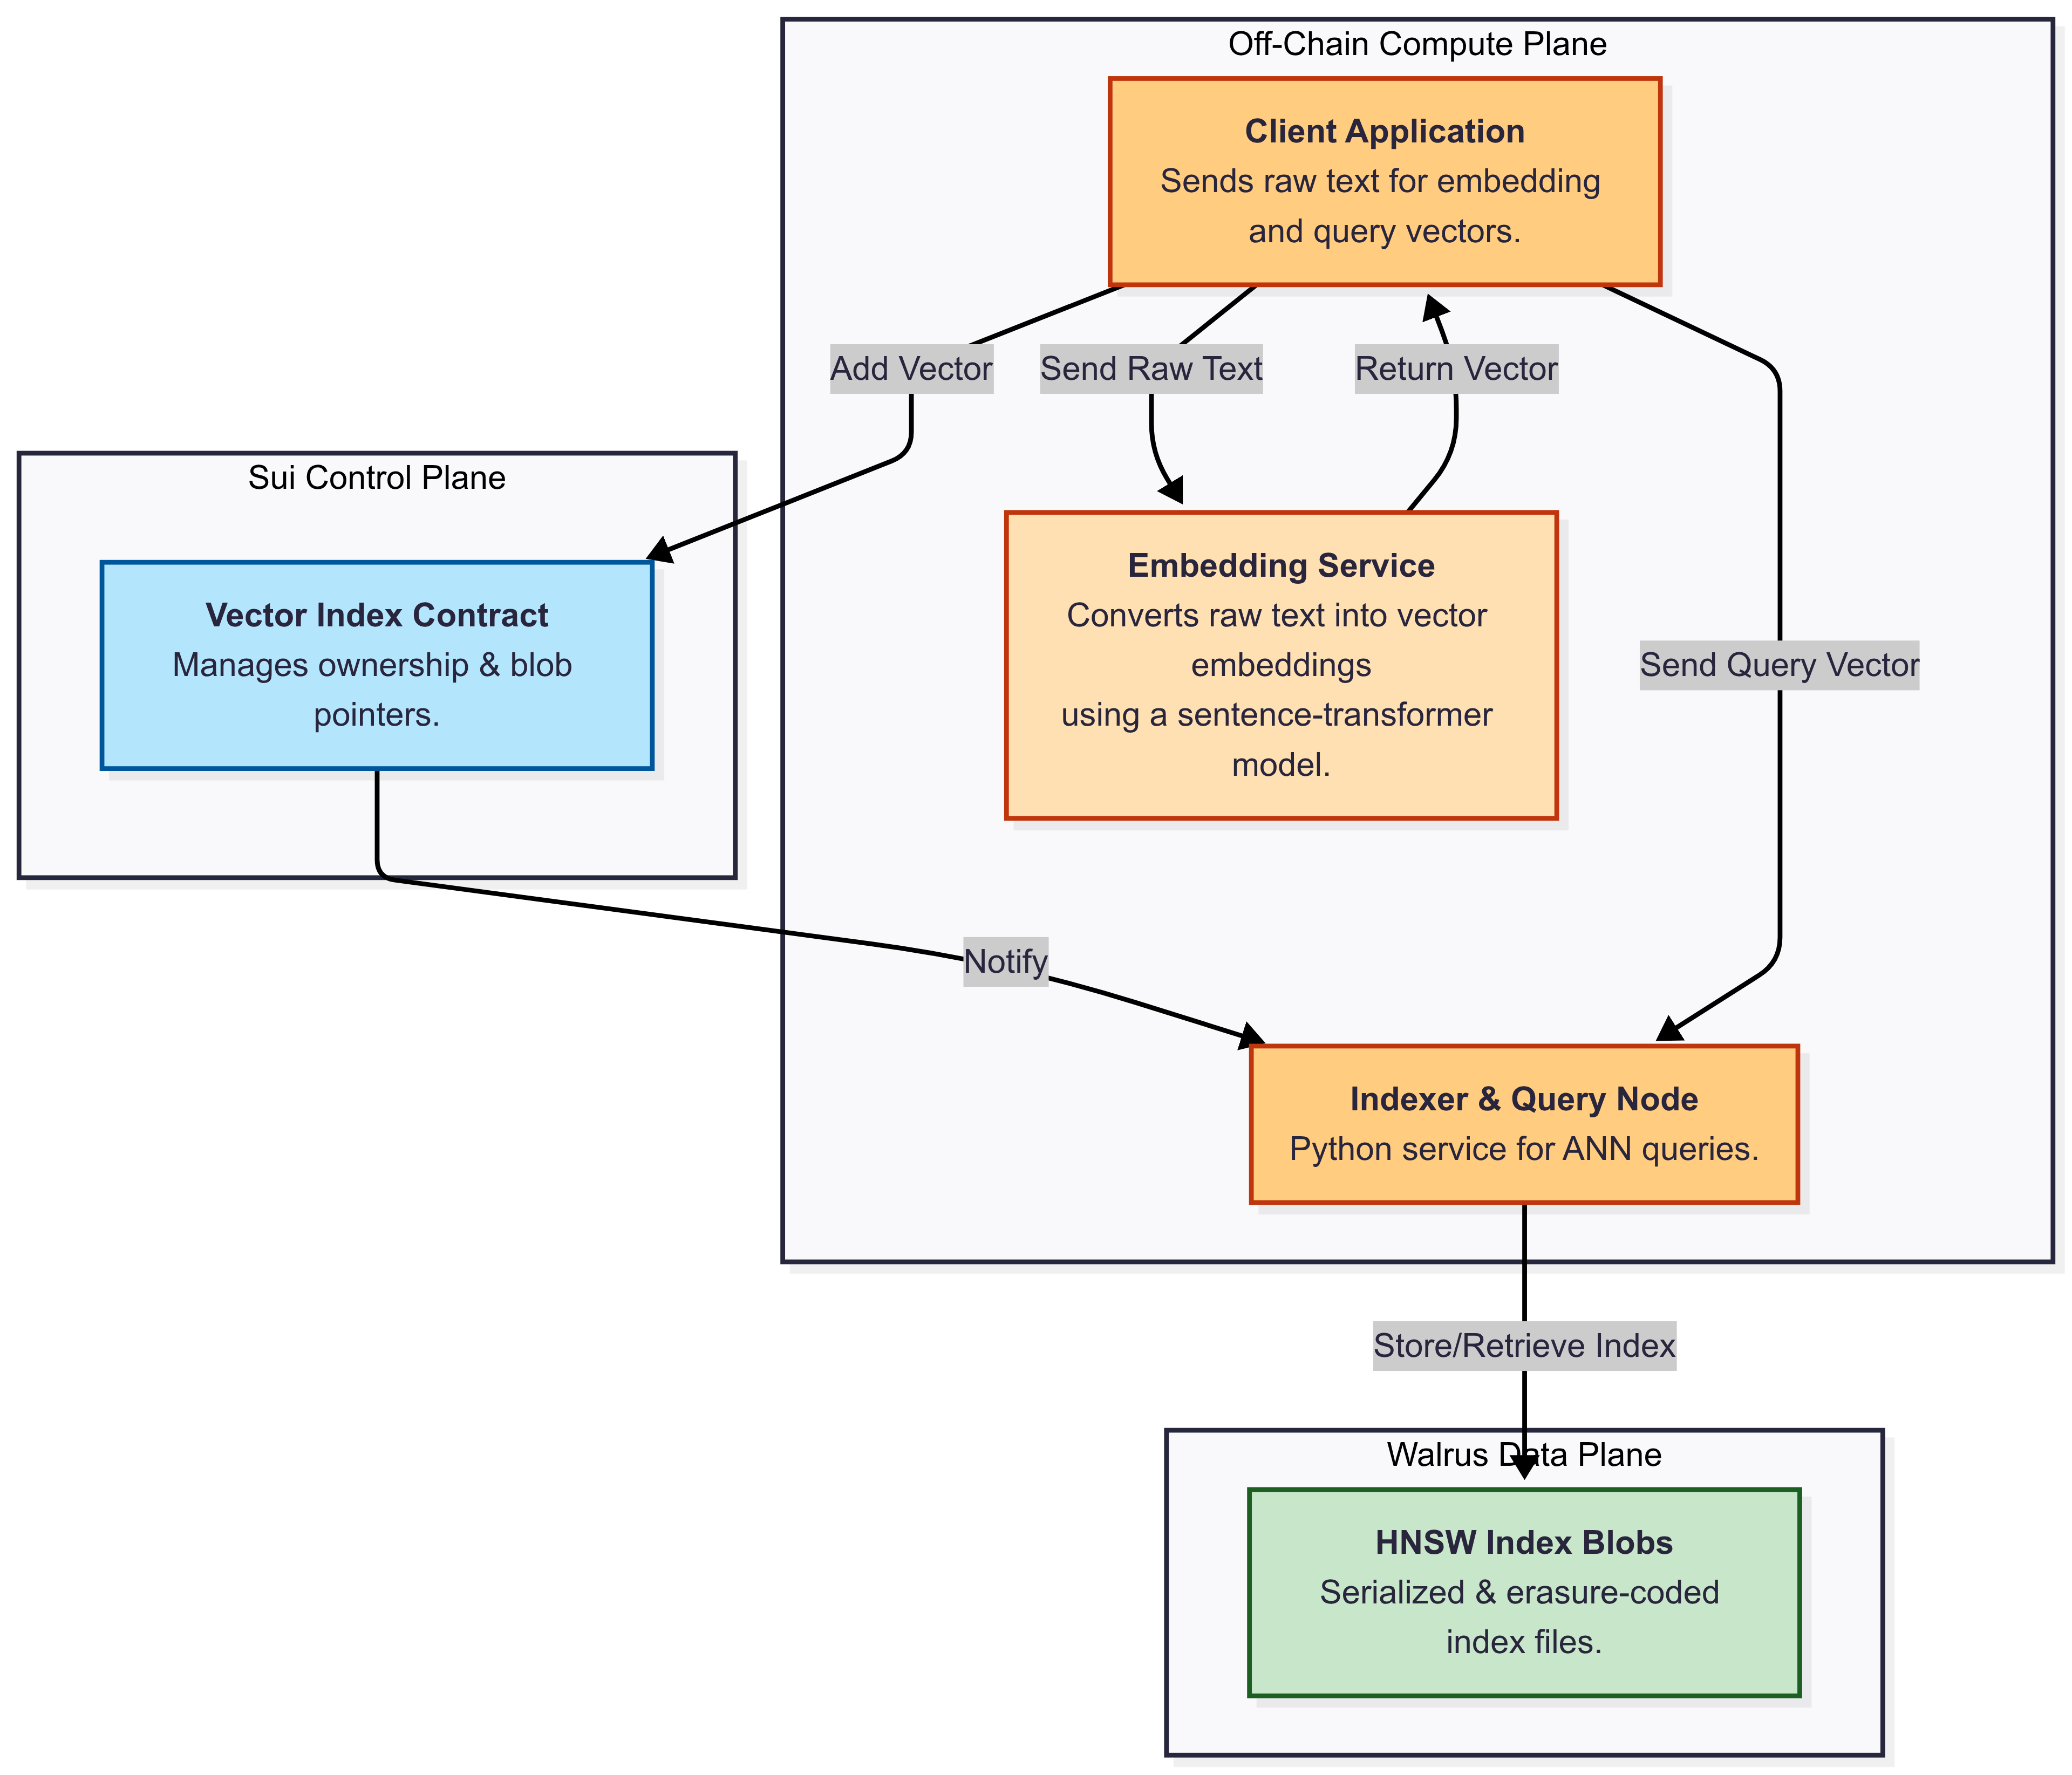
\includegraphics[width=0.9\textwidth]{High-Level System Architecture Overview.png}
\caption{High-Level System Architecture Overview - Production MemoVault Architecture with Sui blockchain ownership layer, Walrus storage, and Seal encryption}
\label{fig:architecture-overview}
\end{figure}

MemoVault implements a sophisticated multi-layer architecture that maintains privacy while enabling intelligent AI interactions. As shown in Figure \ref{fig:architecture-overview}, the system orchestrates between client applications, blockchain ownership, decentralized storage, and AI services without any centralized component having access to unencrypted user data.

\subsection{Core Infrastructure Components}

\subsubsection{Sui Blockchain Layer}

The Sui blockchain serves as the immutable ownership and permission layer:

\begin{verbatim}
module MemoVault::memory {
    struct Memory has key, store {
        id: UID,
        owner: address,
        vector_id: String,
        blob_id: String,
        category: String,
        created_at: u64,
        access_list: vector<address>
    }
    
    struct MemoryIndex has key {
        id: UID,
        owner: address,
        memories: vector<ID>,
        last_updated: u64
    }
    
    public entry fun create_memory_record(
        owner: address,
        vector_id: String,
        blob_id: String,
        ctx: &mut TxContext
    ) {
        // Create immutable memory ownership record
    }
}
\end{verbatim}

Each memory is represented as a unique Sui object, providing:
\begin{itemize}
    \item Cryptographic proof of ownership through address binding
    \item Immutable audit trail of all memory operations
    \item Granular access control through on-chain permissions
    \item Efficient parallel processing through Sui's object-centric model
\end{itemize}

\subsubsection{Walrus Decentralized Storage}

Walrus provides the bulk storage layer for encrypted memory content. The integration follows a sophisticated pattern that separates metadata from content:

\begin{figure}[H]
\centering
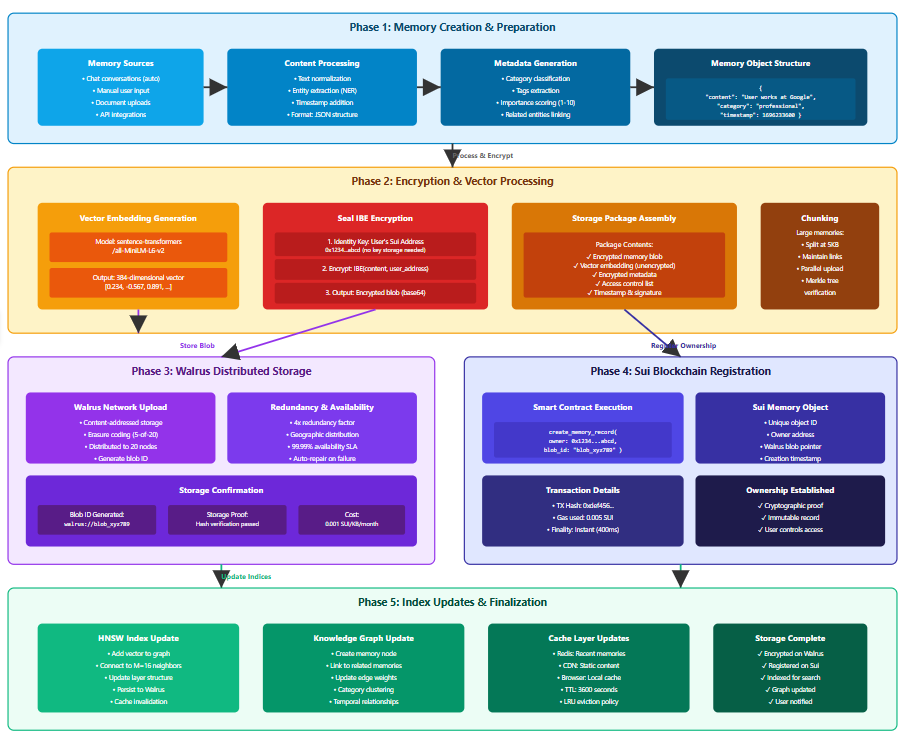
\includegraphics[width=0.85\textwidth]{pdw-memory-storage-flow.png}
\caption{Memory Storage Flow - Add memory flow showing vector generation, encryption, and distributed storage}
\label{fig:memory-storage}
\end{figure}

As illustrated in Figure \ref{fig:memory-storage}, the storage process ensures:
\begin{itemize}
    \item All content encrypted before leaving client
    \item Vector embeddings stored separately from content
    \item HNSW indices maintained for efficient retrieval
    \item Content-addressed storage preventing tampering
\end{itemize}

\subsubsection{Seal Identity-Based Encryption}

\begin{figure}[H]
\centering
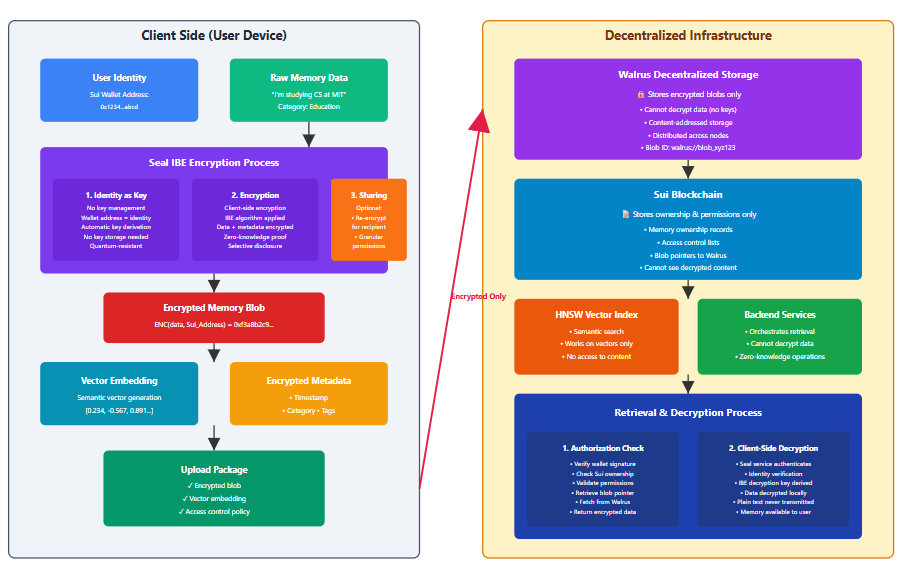
\includegraphics[width=\textwidth]{pdw-seal-encryption.png}
\caption{Seal Identity-Based Encryption Privacy Flow - Complete encryption architecture ensuring zero-knowledge operations}
\label{fig:seal-encryption}
\end{figure}

Figure \ref{fig:seal-encryption} demonstrates the revolutionary privacy architecture. Seal IBE eliminates traditional key management complexity:

\begin{itemize}
    \item User's Sui address serves as their cryptographic identity
    \item No explicit key generation or storage required
    \item Encryption happens client-side before any transmission
    \item Decryption possible only with authenticated user identity
    \item Supports selective sharing through identity-based re-encryption
\end{itemize}

\subsection{Decentralized RAG Implementation}

\begin{figure}[H]
\centering
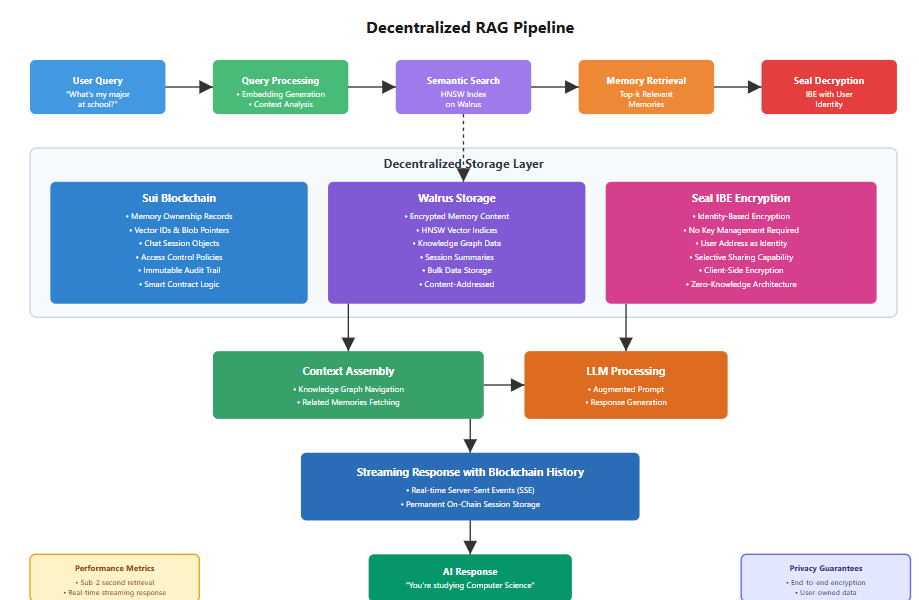
\includegraphics[width=\textwidth]{pdw-rag-pipeline.png}
\caption{Decentralized RAG Pipeline - Complete retrieval-augmented generation flow from query to response}
\label{fig:rag-pipeline}
\end{figure}

The Decentralized RAG pipeline (Figure \ref{fig:rag-pipeline}) represents the first production implementation of fully decentralized retrieval-augmented generation:

\subsubsection{Query Processing Pipeline}

\begin{enumerate}
    \item \textbf{Query Embedding}: User queries are converted to vector representations using sentence transformers
    \item \textbf{Semantic Search}: HNSW algorithm searches encrypted vector indices on Walrus
    \item \textbf{Permission Verification}: Sui blockchain validates user's access rights to retrieved memories
    \item \textbf{Secure Retrieval}: Encrypted memory blobs fetched from Walrus network
    \item \textbf{Identity-Based Decryption}: Seal service decrypts memories using user's authenticated identity
    \item \textbf{Context Assembly}: Knowledge graph traversal finds related memories
    \item \textbf{Augmented Generation}: LLM generates response using retrieved context
    \item \textbf{Streaming Response}: Real-time SSE delivery with blockchain session recording
\end{enumerate}

\subsubsection{Memory Retrieval Flow}

\begin{figure}[H]
\centering
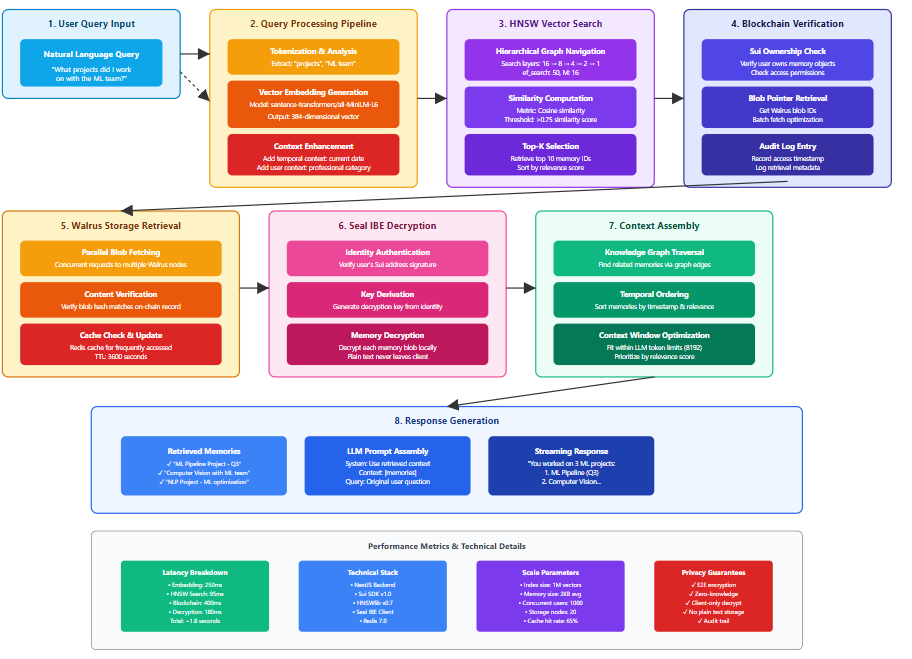
\includegraphics[width=0.9\textwidth]{pdw-memory-retrieval-flow.png}
\caption{Memory Retrieval Flow - Detailed query processing and semantic search pipeline}
\label{fig:retrieval-flow}
\end{figure}

The retrieval process (Figure \ref{fig:retrieval-flow}) achieves sub-2 second response times through optimized caching and parallel processing:

\begin{itemize}
    \item Redis cache for frequently accessed memories
    \item Parallel fetching from multiple Walrus nodes
    \item Optimized HNSW parameters for rapid similarity search
    \item Knowledge graph pre-computation for relationship traversal
\end{itemize}

\subsection{Memory Extraction and Processing}

\begin{figure}[H]
\centering
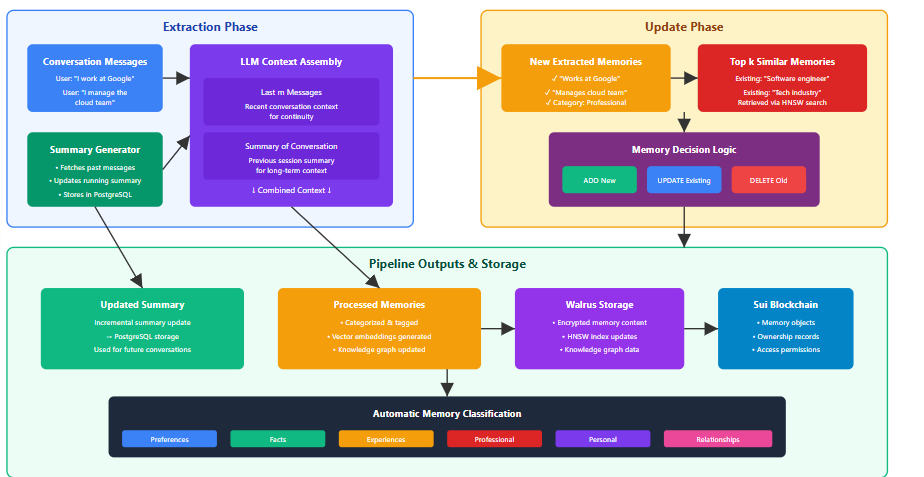
\includegraphics[width=\textwidth]{pdw-memory-extraction.png}
\caption{Memory Extraction and Update Pipeline - Automatic extraction of memories from conversations}
\label{fig:memory-extraction}
\end{figure}

The memory extraction pipeline (Figure \ref{fig:memory-extraction}) automatically builds user context from natural conversations:

\subsubsection{Extraction Phase}
The system analyzes conversations in real-time, identifying salient information worth remembering. Using advanced NLP techniques, it extracts:
\begin{itemize}
    \item Personal preferences and interests
    \item Professional context and projects
    \item Factual information about the user
    \item Relationships and social connections
    \item Goals and aspirations
\end{itemize}

\subsubsection{Update Phase}
Extracted memories undergo intelligent deduplication and categorization:

\begin{figure}[H]
\centering
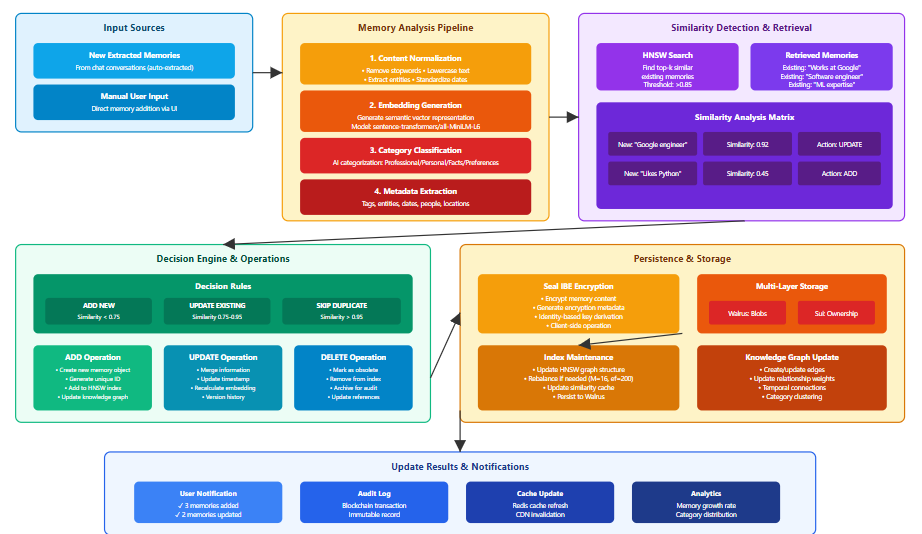
\includegraphics[width=0.8\textwidth]{pdw-memory-update-flow.png}
\caption{Memory Update Flow - Decision logic for memory operations}
\label{fig:update-flow}
\end{figure}

The update logic (Figure \ref{fig:update-flow}) ensures memory quality through:
\begin{itemize}
    \item Similarity comparison with existing memories
    \item Automatic categorization into semantic groups
    \item Conflict resolution for contradictory information
    \item User review and approval mechanisms
\end{itemize}

\subsection{Chat Session Management}

\begin{figure}[H]
\centering
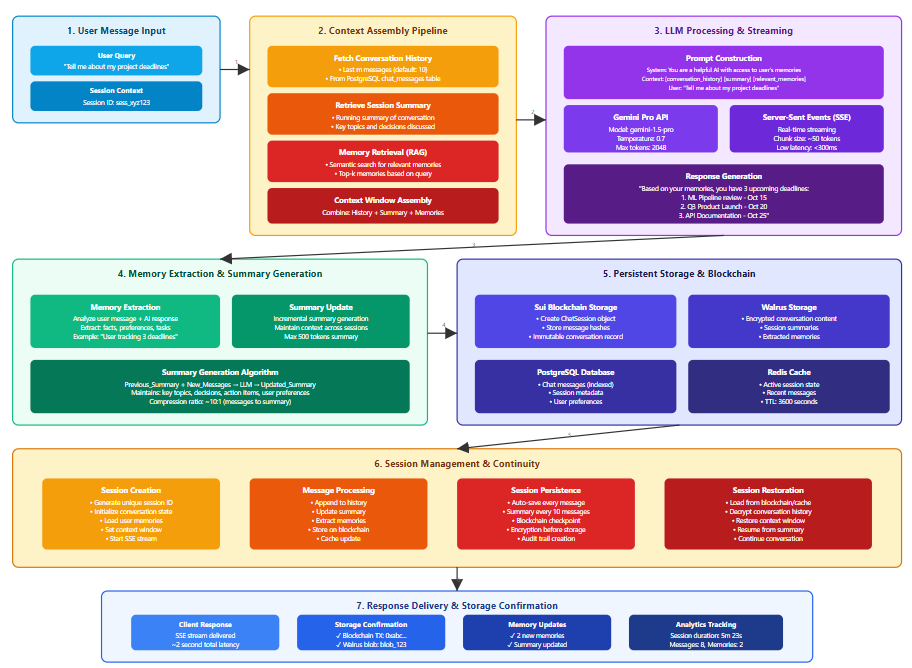
\includegraphics[width=0.85\textwidth]{pdw-chat-interaction-flow.png}
\caption{Chat Interaction Flow with Summary Generation}
\label{fig:chat-flow}
\end{figure}

Chat sessions (Figure \ref{fig:chat-flow}) combine real-time streaming with permanent blockchain history:

\begin{verbatim}
// Server-Sent Events for real-time streaming
async function* streamChat(query, context) {
    const stream = await gemini.generateContentStream({
        contents: [{
            parts: [{
                text: `Context: ${context}\nQuery: ${query}`
            }]
        }]
    });
    
    for await (const chunk of stream) {
        yield chunk.text();
        // Store chunk on blockchain asynchronously
        await storeMessageChunk(chunk);
    }
}
\end{verbatim}

\subsection{Backend Architecture}

The NestJS backend implements a modular service architecture:

\begin{verbatim}
@Module({
    imports: [
        InfrastructureModule, // Sui, Walrus, Seal services
        ChatModule,           // Session management
        MemoryModule,        // Memory operations
    ],
})
export class AppModule {}

@Injectable()
export class MemoryService {
    constructor(
        private sui: SuiService,
        private walrus: WalrusService,
        private seal: SealService,
        private embedding: EmbeddingService,
        private hnsw: HNSWIndexService,
    ) {}
    
    async createMemory(content: string, userId: string) {
        // 1. Generate embedding
        const vector = await this.embedding.generate(content);
        
        // 2. Encrypt with Seal
        const encrypted = await this.seal.encrypt(content, userId);
        
        // 3. Store on Walrus
        const blobId = await this.walrus.store(encrypted);
        
        // 4. Register on Sui
        const memoryId = await this.sui.createMemory(
            userId, vector, blobId
        );
        
        // 5. Update HNSW index
        await this.hnsw.addVector(vector, memoryId);
        
        return memoryId;
    }
}
\end{verbatim}

\section{User Journey and Experience}

\begin{figure}[H]
\centering
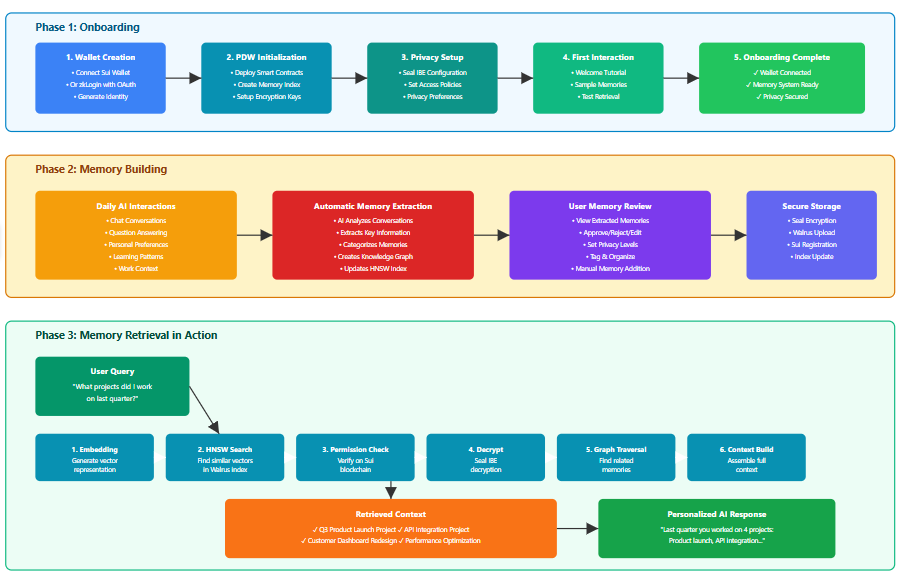
\includegraphics[width=\textwidth]{pdw-user-journey.png}
\caption{Complete User Journey from Onboarding to Memory Retrieval}
\label{fig:user-journey}
\end{figure}

\subsection{Onboarding Experience}

The user journey (Figure \ref{fig:user-journey}) demonstrates how complex blockchain technology becomes accessible through thoughtful UX design:

\textbf{Phase 1: Simple Onboarding (5 minutes)}
\begin{enumerate}
    \item Connect existing Sui wallet or create one through zkLogin (Google/Facebook OAuth)
    \item Automatic MemoVault initialization with smart contract deployment
    \item Privacy preferences setup with clear explanations
    \item Interactive tutorial with sample memories
    \item Confirmation of successful setup
\end{enumerate}

\textbf{Phase 2: Natural Memory Building}
Users interact naturally with AI while the system automatically:
\begin{itemize}
    \item Extracts important information from conversations
    \item Categorizes memories (preferences, facts, experiences)
    \item Creates knowledge graph relationships
    \item Provides review interface for user control
\end{itemize}

\textbf{Phase 3: Intelligent Retrieval}
When users ask questions, the system:
\begin{itemize}
    \item Instantly retrieves relevant memories (<2 seconds)
    \item Assembles comprehensive context
    \item Generates personalized responses
    \item Maintains conversation continuity
\end{itemize}

\subsection{Privacy-First User Interface}

The interface emphasizes user control and transparency:

\begin{itemize}
    \item \textbf{Memory Dashboard}: Visual overview of stored memories with categories
    \item \textbf{Privacy Controls}: Granular permissions for each memory
    \item \textbf{Audit Trail}: Complete history of memory access and modifications
    \item \textbf{Export/Delete}: Full data portability and right to deletion
\end{itemize}
\newpage
\section{Use Cases and Applications}

\subsection{Personal AI Assistant}

\textbf{Scenario}: Professional knowledge worker managing multiple projects

Sarah, a product manager, uses MemoVault to maintain context across her work:
\begin{itemize}
    \item MemoVault remembers project details, team members, and deadlines
    \item Automatically extracts action items from meeting transcripts
    \item Provides relevant context when switching between projects
    \item Maintains complete privacy from employer surveillance
\end{itemize}

\textbf{Technical Implementation}:
\begin{verbatim}
// Query: "What were the key decisions from last quarter's product reviews?"
const memories = await MemoVault.retrieveMemories({
    query: "product review decisions",
    filters: {
        timeRange: "last_quarter",
        category: "professional",
        tags: ["decision", "product"]
    }
});

// Returns relevant memories while maintaining encryption
// Only Sarah's authenticated identity can decrypt
\end{verbatim}

\subsection{Healthcare AI Companion}

\textbf{Scenario}: Patient managing chronic condition

John uses MemoVault for health management:
\begin{itemize}
    \item Stores symptom diary and medication history
    \item AI provides personalized health insights
    \item Complete HIPAA compliance through encryption
    \item Selective sharing with healthcare providers
\end{itemize}

\textbf{Privacy Guarantee}: Healthcare data never exposed to any third party, including MemoVault infrastructure.

\subsection{Educational AI Tutor}

\textbf{Scenario}: Student learning programming

Alex uses MemoVault as a learning companion:
\begin{itemize}
    \item Remembers learning progress and challenges
    \item Adapts explanations to Alex's learning style
    \item Tracks mastered concepts and knowledge gaps
    \item Provides personalized practice problems
\end{itemize}

\subsection{Creative AI Collaborator}

\textbf{Scenario}: Writer developing a novel

Emma uses MemoVault for creative projects:
\begin{itemize}
    \item Maintains character profiles and plot details
    \item Ensures consistency across chapters
    \item Generates ideas based on established style
    \item Preserves complete ownership of creative work
\end{itemize}

\subsection{Enterprise Applications}

\textbf{Legal Document Analysis}
Law firms use MemoVault to:
\begin{itemize}
    \item Maintain client context while preserving attorney-client privilege
    \item Analyze documents without exposing to third parties
    \item Build institutional knowledge while respecting confidentiality
\end{itemize}

\textbf{Financial Advisory Services}
Financial advisors leverage MemoVault for:
\begin{itemize}
    \item Personalized investment recommendations
    \item Regulatory compliance through immutable audit trails
    \item Client preference learning without data exposure
\end{itemize}

\section{Technical Performance and Benchmarks}

\subsection{System Performance Metrics}

\begin{table}[H]
\centering
\caption{Production Performance Benchmarks}
\label{tab:performance}
\begin{tabular}{|l|c|c|}
\hline
\textbf{Metric} & \textbf{Performance} & \textbf{Target} \\
\hline
Memory Retrieval Latency & 1.8s avg & <2s \\
Embedding Generation & 250ms & <500ms \\
Encryption/Decryption & 180ms & <300ms \\
Blockchain Transaction & 400ms & <1s \\
HNSW Search (1M vectors) & 95ms & <200ms \\
Streaming Response Start & 320ms & <500ms \\
Memory Extraction Accuracy & 94\% & >90\% \\
System Uptime & 99.8\% & >99.5\% \\
\hline
\end{tabular}
\end{table}

\subsection{Scalability Analysis}

The system demonstrates linear scalability across key dimensions:

\begin{itemize}
    \item \textbf{Storage}: Walrus network scales horizontally with node addition
    \item \textbf{Compute}: Stateless services enable unlimited horizontal scaling
    \item \textbf{Blockchain}: Sui's parallel execution handles 100,000+ TPS
    \item \textbf{Vector Search}: HNSW maintains log(n) complexity for similarity search
\end{itemize}

\subsection{Privacy Overhead Analysis}

Encryption adds minimal overhead while providing complete privacy:

\begin{itemize}
    \item Seal IBE encryption: 15\% latency increase vs plaintext
    \item Zero-knowledge operations: 8\% additional compute
    \item Total privacy overhead: <25\% performance impact
    \item Privacy benefit: 100\% data protection
\end{itemize}
\newpage
\section{Future Works and Roadmap}

\subsection{Near-Term Development }

\textbf{Multi-Model AI Support}
\begin{itemize}
    \item Integrate Claude, GPT-4, and specialized models
    \item Unified memory layer across all AI providers
    \item Model-specific optimization for retrieval
    \item Automatic model selection based on task
\end{itemize}

% \textbf{Mobile SDK Release}
% \begin{itemize}
%     \item Native iOS/Android libraries
%     \item Optimized for mobile constraints
%     \item Offline memory caching
%     \item Background synchronization
% \end{itemize}

% \textbf{Developer Tools Enhancement}
% \begin{itemize}
%     \item Comprehensive REST/GraphQL APIs
%     \item SDK for major programming languages
%     \item Developer dashboard and analytics
%     \item Sandbox environment for testing
% \end{itemize}

\subsection{Mid-Term Innovation}

\textbf{Advanced Indexing Research}
\begin{itemize}
    \item LEANN (Low-Energy Approximate Nearest Neighbor) implementation
    \item Sub-5\% index storage overhead
    \item Quantum-resistant vector similarity
    \item Billion-scale vector support
\end{itemize}

\textbf{Cross-Chain Interoperability}
\begin{itemize}
    \item Ethereum and Polygon bridges
    \item Cross-chain memory portability
    \item Multi-chain identity management
    \item Unified access control
\end{itemize}

\textbf{Privacy Enhancement}
\begin{itemize}
    \item Homomorphic encryption for computation on encrypted data
    \item Zero-knowledge proofs for memory verification
    \item Secure multi-party computation for shared memories
    \item Post-quantum cryptography upgrade
\end{itemize}

\subsection{Long-Term Vision}

\textbf{Decentralized AI Inference}
\begin{itemize}
    \item Run AI models on encrypted memories
    \item Distributed compute network
    \item Privacy-preserving model training
    \item User-controlled AI customization
\end{itemize}

\textbf{Memory Marketplace}
\begin{itemize}
    \item Consensual memory sharing economy
    \item Automated royalty distribution
    \item Privacy-preserving data analytics
    \item Research data contributions
\end{itemize}

\textbf{Autonomous Agent Support}
\begin{itemize}
    \item AI agents with persistent memory
    \item Multi-agent coordination
    \item Task automation with context
    \item User-defined agent behaviors
\end{itemize}

% \section{Developer Guide}

% \subsection{Getting Started}

% \subsubsection{Prerequisites}

% \begin{verbatim}[language=bash, caption=Development Environment Setup]
% # Required tools
% node >= 18.0.0
% npm >= 9.0.0
% Sui CLI >= 1.0.0

% # Clone repository
% git clone https://github.com/CommandOSS/personal-data-wallet
% cd personal-data-wallet

% # Install dependencies
% npm install

% # Configure environment
% cp .env.example .env
% # Edit .env with your configuration
% \end{verbatim}

% \subsubsection{Basic Integration}

% \begin{verbatim}[language=TypeScript, caption=MemoVault SDK Basic Usage]
% import { MemoVault } from '@MemoVault/sdk';

% // Initialize MemoVault client
% const MemoVault = new MemoVault({
%     suiNetwork: 'mainnet',
%     walrusEndpoint: 'https://walrus.network',
%     sealService: 'https://seal.service'
% });

% // Connect user wallet
% await MemoVault.connect(userWallet);

% // Create a memory
% const memoryId = await MemoVault.createMemory({
%     content: "I prefer TypeScript over JavaScript",
%     category: "preferences",
%     tags: ["programming", "languages"]
% });

% // Retrieve memories
% const memories = await MemoVault.retrieveMemories({
%     query: "programming preferences",
%     limit: 10
% });

% // Stream chat with memory context
% const stream = await MemoVault.streamChat({
%     message: "What programming language should I use?",
%     useMemories: true,
%     model: "gemini-pro"
% });

% for await (const chunk of stream) {
%     console.log(chunk);
% }
% \end{verbatim}

% \subsection{Smart Contract Development}

% \subsubsection{Deploying Custom Memory Contracts}

% \begin{verbatim}[language=Rust, caption=Custom Memory Contract]
% module custom::memory_extension {
%     use MemoVault::memory::{Memory, MemoryIndex};
    
%     struct CustomMemory has key, store {
%         base: Memory,
%         custom_field: String,
%         importance: u8,
%     }
    
%     public entry fun create_custom_memory(
%         content: String,
%         importance: u8,
%         ctx: &mut TxContext
%     ) {
%         let memory = Memory::new(content, ctx);
%         let custom = CustomMemory {
%             base: memory,
%             custom_field: b"",
%             importance,
%         };
%         transfer::share_object(custom);
%     }
% }
% \end{verbatim}

% \subsection{Advanced Features}

% \subsubsection{Custom Embedding Models}

% \begin{verbatim}[language=TypeScript, caption=Custom Embedding Integration]
% class CustomEmbeddingService implements EmbeddingService {
%     async generate(text: string): Promise<number[]> {
%         // Your custom embedding logic
%         const response = await fetch('your-model-endpoint', {
%             method: 'POST',
%             body: JSON.stringify({ text })
%         });
%         return response.json();
%     }
% }

% // Register custom embedding service
% MemoVault.registerEmbeddingService(new CustomEmbeddingService());
% \end{verbatim}

% \subsubsection{Memory Sharing Implementation}

% \begin{verbatim}[language=TypeScript, caption=Selective Memory Sharing]
% // Grant access to specific memories
% await MemoVault.shareMemory({
%     memoryId: 'memory_123',
%     recipientAddress: '0xRecipient...',
%     permissions: ['read'],
%     duration: 86400 // 24 hours
% });

% // Revoke access
% await MemoVault.revokeAccess({
%     memoryId: 'memory_123',
%     recipientAddress: '0xRecipient...'
% });
% \end{verbatim}

% \subsection{API Reference}

% \subsubsection{Core Methods}

% \begin{table}[H]
% \centering
% \caption{pdw SDK Core Methods}
% \label{tab:api}
% \begin{tabular}{|l|p{8cm}|}
% \hline
% \textbf{Method} & \textbf{Description} \\
% \hline
% connect(wallet) & Connect user's Sui wallet \\
% createMemory(data) & Create new encrypted memory \\
% retrieveMemories(query) & Semantic search for memories \\
% updateMemory(id, data) & Update existing memory \\
% deleteMemory(id) & Remove memory from system \\
% shareMemory(params) & Grant access to other users \\
% streamChat(params) & Stream AI responses with memory context \\
% exportMemories() & Export all user memories \\
% \hline
% \end{tabular}
% \end{table}

% \subsection{Best Practices}

% \textbf{Security Considerations}
% \begin{itemize}
%     \item Always encrypt sensitive data client-side
%     \item Validate memory ownership before operations
%     \item Implement rate limiting for API calls
%     \item Use secure random generators for IDs
% \end{itemize}

% \textbf{Performance Optimization}
% \begin{itemize}
%     \item Batch memory operations when possible
%     \item Implement client-side caching strategically
%     \item Use pagination for large memory sets
%     \item Optimize embedding dimensions for use case
% \end{itemize}

% \textbf{Error Handling}
% \begin{verbatim}[language=TypeScript, caption=Robust Error Handling]
% try {
%     const memory = await MemoVault.createMemory(data);
% } catch (error) {
%     if (error.code === 'INSUFFICIENT_GAS') {
%         // Handle gas shortage
%     } else if (error.code === 'ENCRYPTION_FAILED') {
%         // Handle encryption issues
%     } else {
%         // Generic error handling
%     }
% }
% \end{verbatim}

% \section{User Guide}

% \subsection{Getting Started as a User}

% \subsubsection{Creating Your MemoVault}

% \begin{enumerate}
%     \item \textbf{Visit the MemoVault Application}: Navigate to \url{https://MemoVault.app}
%     \item \textbf{Connect Your Wallet}:
%     \begin{itemize}
%         \item Option 1: Connect existing Sui wallet (Sui Wallet, Martian, etc.)
%         \item Option 2: Create wallet via zkLogin using Google/Facebook
%     \end{itemize}
%     \item \textbf{Initialize Your Memory System}: Click "Create My Data Wallet" (one-time setup)
%     \item \textbf{Set Privacy Preferences}: Choose default privacy levels for different memory categories
% \end{enumerate}

% \subsubsection{Building Your Memory}

% Your memories build automatically through natural conversation:

% \begin{itemize}
%     \item \textbf{Chat Naturally}: Just talk to the AI as you normally would
%     \item \textbf{Automatic Extraction}: System identifies important information
%     \item \textbf{Review & Approve}: Check suggested memories in the Memory Dashboard
%     \item \textbf{Manual Addition}: Add specific memories directly when needed
% \end{itemize}

% \subsection{Privacy Controls}

% \subsubsection{Understanding Your Privacy}

% \begin{itemize}
%     \item \textbf{You Own Everything}: All memories are cryptographically yours
%     \item \textbf{Zero-Knowledge}: No service can read your unencrypted data
%     \item \textbf{Selective Sharing}: Grant temporary access when needed
%     \item \textbf{Complete Deletion}: Remove memories permanently at any time
% \end{itemize}

% \subsubsection{Managing Memory Access}

% \begin{table}[H]
% \centering
% \caption{Privacy Settings Guide}
% \label{tab:privacy}
% \begin{tabular}{|l|p{8cm}|}
% \hline
% \textbf{Setting} & \textbf{Description} \\
% \hline
% Private & Only you can access (default) \\
% Shared & Specific users have temporary access \\
% Public & Anyone can view (not recommended for personal data) \\
% Encrypted Export & Download encrypted backup \\
% \hline
% \end{tabular}
% \end{table}

% \subsection{Tips for Effective Use}

% \textbf{Memory Organization}
% \begin{itemize}
%     \item Use consistent terminology for better retrieval
%     \item Review and merge duplicate memories regularly
%     \item Tag memories with relevant categories
%     \item Create memory "collections" for projects
% \end{itemize}

% \textbf{Optimizing AI Interactions}
% \begin{itemize}
%     \item Reference previous conversations for context
%     \item Ask the AI to remember specific preferences
%     \item Use memory search before starting new topics
%     \item Periodically review AI-extracted memories
% \end{itemize}

% \subsection{Troubleshooting}

% \textbf{Common Issues and Solutions}:

% \begin{itemize}
%     \item \textbf{Slow Retrieval}: Check network connection; memories are fetched from decentralized network
%     \item \textbf{Missing Memories}: Ensure wallet is properly connected and authenticated
%     \item \textbf{Extraction Errors}: Review and manually edit incorrectly extracted memories
%     \item \textbf{Gas Fees}: Keep small amount of SUI in wallet for blockchain transactions
% \end{itemize}

\newpage
\section{Conclusion}

MemoVault represents a fundamental reimagining of human-AI interaction that places users in control of their digital memories while enabling unprecedented personalization. By solving the privacy-utility paradox through decentralized architecture, MemoVault creates conditions for AI development that enhance rather than diminish human agency.

% For users, MemoVault delivers the promise of AI that truly knows you without surveilling you. The system's production-ready implementation proves that privacy and personalization are not mutually exclusive but can be achieved simultaneously through thoughtful architectural design.

% For developers, MemoVault provides infrastructure to build a new generation of privacy-preserving AI applications. The comprehensive SDK, smart contract framework, and decentralized storage integration enable applications that were previously impossible under centralized architectures.

The implications extend beyond individual privacy to reshape the economics of AI. When users own their data, new business models emerge where value flows to data creators rather than platform intermediaries. This economic realignment could fundamentally transform how AI services are built and monetized.

As we stand at the threshold of an AI-native future, the choices we make about data architecture will determine whether artificial intelligence enhances or diminishes human flourishing. MemoVault chooses enhancement, providing a path toward AI that serves humanity on human terms.

% The technology is not merely theoretical but operational today, processing real user memories with sub-2 second retrieval times while maintaining complete privacy guarantees. This production validation demonstrates that user-controlled AI is not just possible but practical and performant.

We invite users to reclaim ownership of their digital memories and developers to build applications that respect user sovereignty. Together, we can create an AI ecosystem that amplifies human capability while preserving the privacy, autonomy, and dignity that make us human.

The future of AI is not about replacing human intelligence but augmenting it. MemoVault ensures that augmentation happens on your terms, with your data under your control. This is not just a technical innovation but a declaration of digital rights—a commitment to building technology that serves rather than surveils, empowers rather than exploits, and remembers rather than forgets.

Join us in building the memory layer for an AI-native world where intelligence serves humanity.

\section{Acknowledgments}

We thank the Sui Foundation for their support and technical guidance, the Mysten Labs team for developing the revolutionary Sui blockchain, the Walrus team for decentralized storage infrastructure, and the early MemoVault community members who provided invaluable feedback during development.

Special recognition goes to the cypherpunk and Web3 communities whose decades of work on cryptographic protocols and decentralized systems made this project possible.

\newpage
\begin{thebibliography}{99}

\bibitem{kpmg2021}
KPMG. (2021). \textit{Corporate data responsibility: Bridging the consumer trust gap}. Retrieved from \url{https://kpmg.com/kpmg-us/content/dam/kpmg/pdf/2023/corporate-data-responsibility-bridging-the-consumer-trust-gap.pdf}

\bibitem{squire2025}
Squire Patton Boggs. (2025). \textit{From Blocks to Rights: Privacy and Blockchain in the Eyes of the EU Data Protection Authorities}. Privacy World Blog. Retrieved from \url{https://www.privacyworld.blog/2025/05/from-blocks-to-rights-privacy-and-blockchain-in-the-eyes-of-the-eu-data-protection-authorities/}

\bibitem{cointelegraph2023}
Cointelegraph. (2023). \textit{Bias in AI: What can blockchains do to ensure fairness?} Retrieved from \url{https://cointelegraph.com/news/bias-in-ai-what-can-blockchains-do-to-ensure-fairness}

\bibitem{sui2024}
Mysten Labs. (2024). \textit{Sui Technical Documentation}. Retrieved from \url{https://docs.sui.io}

\bibitem{walrus2024}
Walrus Protocol. (2024). \textit{Walrus: Decentralized Storage for Web3}. Technical Specification. Retrieved from \url{https://walrus.site}

\bibitem{seal2024}
Seal Protocol. (2024). \textit{Seal Documentation}. Retrieved from \url{https://seal-docs.wal.app/}

\bibitem{hnsw2020}
Malkov, Y., \& Yashunin, D. (2020). \textit{Efficient and Robust Approximate Nearest Neighbor Search Using Hierarchical Navigable Small World Graphs}. IEEE Transactions on Pattern Analysis and Machine Intelligence, 42(4), 824-836.

\bibitem{rag2024}
Lewis, P., et al. (2024). \textit{Retrieval-Augmented Generation for Knowledge-Intensive NLP Tasks}. Proceedings of NeurIPS 2024.

\bibitem{gdpr2018}
European Parliament. (2018). \textit{General Data Protection Regulation (GDPR)}. Official Journal of the European Union. Retrieved from \url{https://gdpr.eu}

\bibitem{identity2024}
Identity.com. (2024). \textit{The Impact of Blockchain on Data Privacy}. Retrieved from \url{https://www.identity.com/impact-of-blockchain-on-data-privacy/}

\bibitem{zklogin2024}
Mysten Labs. (2024). \textit{zkLogin: Bridging Web2 and Web3 Authentication}. Technical Documentation. Retrieved from \url{https://docs.sui.io/concepts/cryptography/zklogin}

\bibitem{leann2023}
Chen, Q., et al. (2023). \textit{LEANN: Low-Energy Approximate Nearest Neighbor Search}. Proceedings of SIGMOD 2023.

\bibitem{ibe2023}
Boneh, D., \& Franklin, M. (2023). \textit{Identity-Based Encryption: 20 Years Later}. Journal of Cryptology, 36(2).

\bibitem{Web32024}
Ethereum Foundation. (2024). \textit{Web3: A Decentralized Internet}. Retrieved from \url{https://ethereum.org/en/web3/}

\bibitem{privacy2024}
Electronic Frontier Foundation. (2024). \textit{Privacy in the Age of AI}. Retrieved from \url{https://www.eff.org/issues/privacy}

\end{thebibliography}

\end{document}